% ****** Start of file aipsamp.tex ******
%
%   This file is part of the AIP files in the AIP distribution for REVTeX 4.
%   Version 4.1 of REVTeX, October 2009
%
%   Copyright (c) 2009 American Institute of Physics.
%
%   See the AIP README file for restrictions and more information.
%
% TeX'ing this file requires that you have AMS-LaTeX 2.0 installed
% as well as the rest of the prerequisites for REVTeX 4.1
% 
% It also requires running BibTeX. The commands are as follows:
%
%  1)  latex  aipsamp
%  2)  bibtex aipsamp
%  3)  latex  aipsamp
%  4)  latex  aipsamp
%
% Use this file as a source of example code for your aip document.
% Use the file aiptemplate.tex as a template for your document.
\documentclass[%
 aip,
% jmp,
% bmf,
% sd,
% rsi,
 amsmath,amssymb,
%preprint,%
 reprint,%
%author-year,%
%author-numerical,%
% Conference Proceedings
]{revtex4-1}

\usepackage{graphicx}% Include figure files
\usepackage{dcolumn}% Align table columns on decimal point
\usepackage{bm}% bold math
%\usepackage[mathlines]{lineno}% Enable numbering of text and display math
%\linenumbers\relax % Commence numbering lines

\usepackage[utf8]{inputenc}
\usepackage[T1]{fontenc}
\usepackage{mathptmx}
\usepackage{etoolbox}

\usepackage{amsmath}
\DeclareMathOperator*{\argmin}{arg\,min}

%% Apr 2021: AIP requests that the corresponding 
%% email to be moved after the affiliations
\makeatletter
\def\@email#1#2{%
 \endgroup
 \patchcmd{\titleblock@produce}
  {\frontmatter@RRAPformat}
  {\frontmatter@RRAPformat{\produce@RRAP{*#1\href{mailto:#2}{#2}}}\frontmatter@RRAPformat}
  {}{}
}%
\makeatother
\begin{document}

\preprint{AIP/123-QED}

\title[BASS for Bayesian Optimization]{BASS as a Surrogate Model for Bayesian Optimization}
% Force line breaks with \\
\author{Adrian Tame Jacobo}
 \altaffiliation{Instituto Tecnológico Autónomo de México}%Lines break automatically or can be forced with \\
 \email{atamejac@itam.mx}


\date{\today}% It is always \today, today,
             %  but any date may be explicitly specified

\begin{abstract}
The underlying foundation on which Bayesian Optimization is built are Gaussian Processes. Through repeated sampling, we generate a posterior which is a approximation of the function that we are evaluating. One of the limitations of Gaussian Processes is their inability to approximate solution values when the variables are discrete or categorical. In this paper, we present an extension to the traditional Bayesian Optimization framework, where we use an underlying BASS function instead of a Gaussian Process for curve approximation. We present some references to relevant theory, the changes we made, and a one dimensional implementation in R. 
\end{abstract}

\maketitle

\begin{quotation}
This article is a proof of concept for the idea of changing the underlying surrogate model in Bayesian optimization to something that can still fulfil the same role, but provide more flexibility. While Gaussian Processes preforms better in problems where all the inputs are real numbers, the problem is that this technique cannot be applied or extended to cases where the parameters are categorical or discrete. Bayesian Adaptive Regression Splines (BASS) models are well suited to fit these types of problems though, even if their convergence is not as fast. they provide a solution for these specific families of cases, where tuning mixed hyper-parameters is the goal. 
\end{quotation}

\section{\label{sec:level1}Overview of Bayesian Optimization}

Bayesian Optimization exists because sometimes the functions in some applications are incredibly hard or costly to evaluate. This leads to a problem with applying traditional optimization methods, where the number of iterations that the algorithm runs are not necessarily correlated with a better approximation. One of the solutions to this are Bayesian optimization methods, which are made to also minimize the effective number of iterations needed to find local minima or maxima. We lead the reader to \onlinecite{frazier2018tutorial} for a more detailed and nuanced description of Bayesian Optimization, where most of what we wrote on this section is based on. 

For our purposes, it is sufficient to say that Bayesian Optimization is a class of machine learning based methods that solve the problem 
\[ \max_{x \in A} f(x) \]
where $f(x)$ is a black box function, and we apply derivative-free global optimization methods to solve it. The method we present in this paper is one that is more a proof of concept than a finalized algorithm, as the method is only shown for one dimensional problems that are continuous and not discrete, but, it can be extended to more than one dimension with mixed discrete and continuous inputs. 

There are two primary components that these methods are based on: a method for statistical inference, which in the traditional case is Gaussian process regression; and an acquisition function for deciding where to sample, which is often expected improvement. Each of these components serve a specific purpose, and while the acquisition function tells us where to go next, the statistical inference method generates a posterior or approximation to $f(x)$ at different values of the target space. One of the main reasons Gaussian processes are used in this area is because they not only provide a mean of the expected values of the function, but also a variance. This allows us to measure our uncertainty at different points in the function, and as such, guides our evaluation of new points to sample. 

\begin{figure}
	\centering
	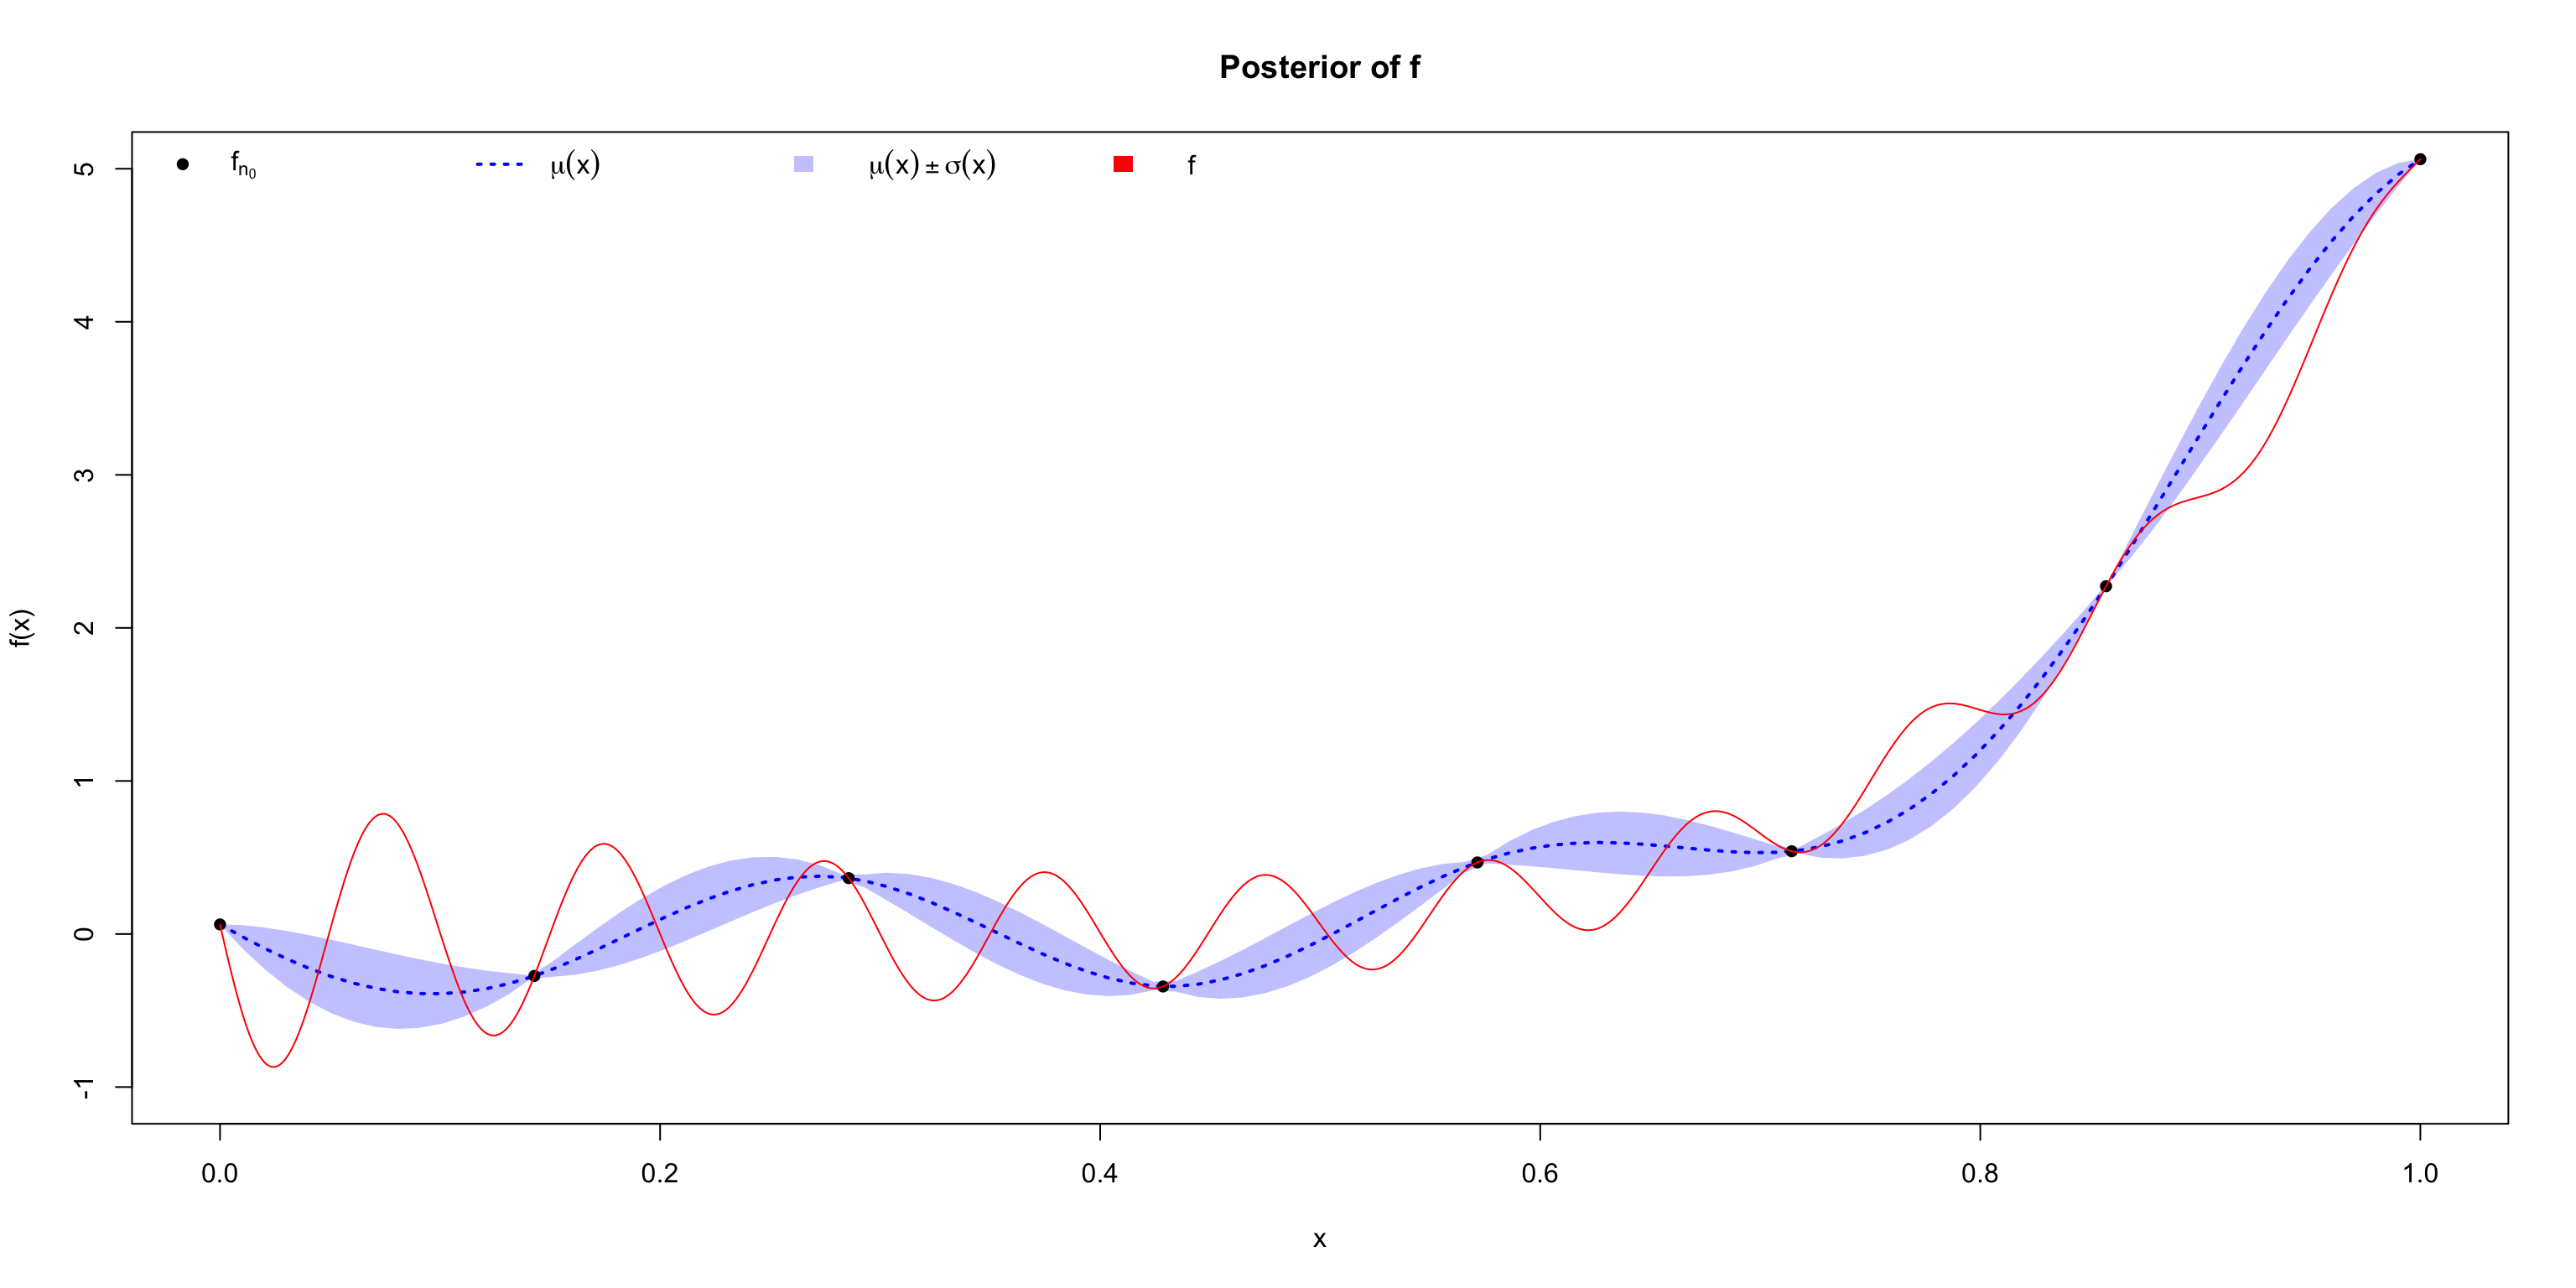
\includegraphics[width=8cm]{Figures/GP8.png}
	\caption{A Gaussian process posterior approximation to the Gramacy and Lee function \cite{gramacy2012cases} with 8 evaluations.}
	\label{gp1}
\end{figure}

\section{Bayesian Adaptive Spline Surface Models}

Bayesian Adaptive Spline Surface (BASS) models are an extension of the family of non parametric regression models of which multivariate adaptive regression splines (MARS) was the first developed in 1991 and is the most basic \cite{friedman1991multivariate}. MARS is an extension of linear models, where interactions between variables and non linearities are modelled automatically. 

The extension of this model of interest is the BMARS model. As the authors state in \cite{denison1998bayesian}, the aim of BMARS is to provide a Bayesian model that mimics the MARS procedure. This is done by considering the number of basis functions, along with their type, the coefficients and their form, random. Then, a suitable MCMC algorithm, in this case reversible jump monte carlo \cite{green1995reversible}, is used to calculate a suitable posterior for the problem. The great advantage to RJMCMC over other MCMC techniques is that the number of parameters can be variable, and as such, is a great basis for the type of analysis that is necessary for models in the MARS class. 

BASS models are an adaptation of BMARS models that include some efficiency improvements for posterior sampling alongside parallel tempering for better posterior exploration \cite{francom2020bass}. For our purposes though, the most significant improvement is that it allows the use of categorical variables alongside some continuous variables. This is incredibly useful in the context of hyper-parameter optimization, where there are generally some categorical variables such as polynomial degree, smoothing, etc. While we remain in the one dimensional case and this improvement is not necessarily useful, the multi dimensional case will benefit greatly from this improvement. 

A detailed rundown of the model, its priors, and its construction in general can be seen in \cite{francom2020bass}, but, we include the definition of the model presented in that work for completeness. 

Let $y_i$ denote the dependent variable and $\boldsymbol{x}_i$ denote a vector of $p$ independent variables, with $i = 1, \ldots, n$. Without loss of generality, let each independent variable be scaled to be between
zero and one. We model $y_i$ as 
\[ y_i = f(\boldsymbol{x}_i) + \epsilon_i, \, \, \epsilon_i \sim \mathcal{N}(0,\sigma^2) \]
\[ f(\boldsymbol{x}) = a_0 + \sum_{m=1}^{M} a_m B_m(\boldsymbol{x}) \]
\[ B_m(\boldsymbol{x}) = \prod_{k=1}^{K_m} g_{km} [s_{km}(\boldsymbol{x}_{v_{km}} - t_{km}) ]^\alpha_+ \]

The only difference between this setup and that of MARS and BMARS is the inclusion of the constant $g_{km}$ in each element of the tensor product. This term is $g_{km}=[s_{km}(\boldsymbol{x}_{v_{km}} - t_{km}) ]^\alpha_+$, where $s_{km} \in \{-1,1\}$ is referred to as the sign, $t_{km}\in [0,1]$ is a knot, $v_{km}$ selects a variable, $K_m$ is the degree of interaction, and $\alpha$ determines the degree of the polynomial splines. This normalizes the basis functions so that the basis coefficients $a_1, \ldots, a_M$ are on the same scale, making computations more stable.

\section{BASS for Bayesian Optimization}

The main problem we had adapting the BASS method to a Bayesian optimization framework was that most everything is built with the underlying Gaussian Process in mind. For starters, the data points are interpolated when using Gaussian processes, while we only have curve fitting with BASS. This is not a problem though, because for the purposes of finding minima and maxima, we are not trying to fit a curve perfectly and understand the behaviour of the target function everywhere. 

This problem was noticeable for example in the calculation of the variance that we assign different points on the curve. With Gaussian processes, the nature of the distribution assigns a certain variance to points outside of the interpolation ones, as can be seen in Figure \ref{gp1}. We do not have that behaviour in BASS, so we built something similar, which is visualized in Figure \ref{gram8}. We decided that a simple way to calculate variance on the points we are approximating is to assign it depending on the distance to the nearest interpolation point on the mesh. This means that the further a point is from an already evaluated point, we assign a higher variance to it. Therefore, the midpoints between current points we have already evaluated are the candidates for the next round of iterations. 

\begin{figure}
	\centering
	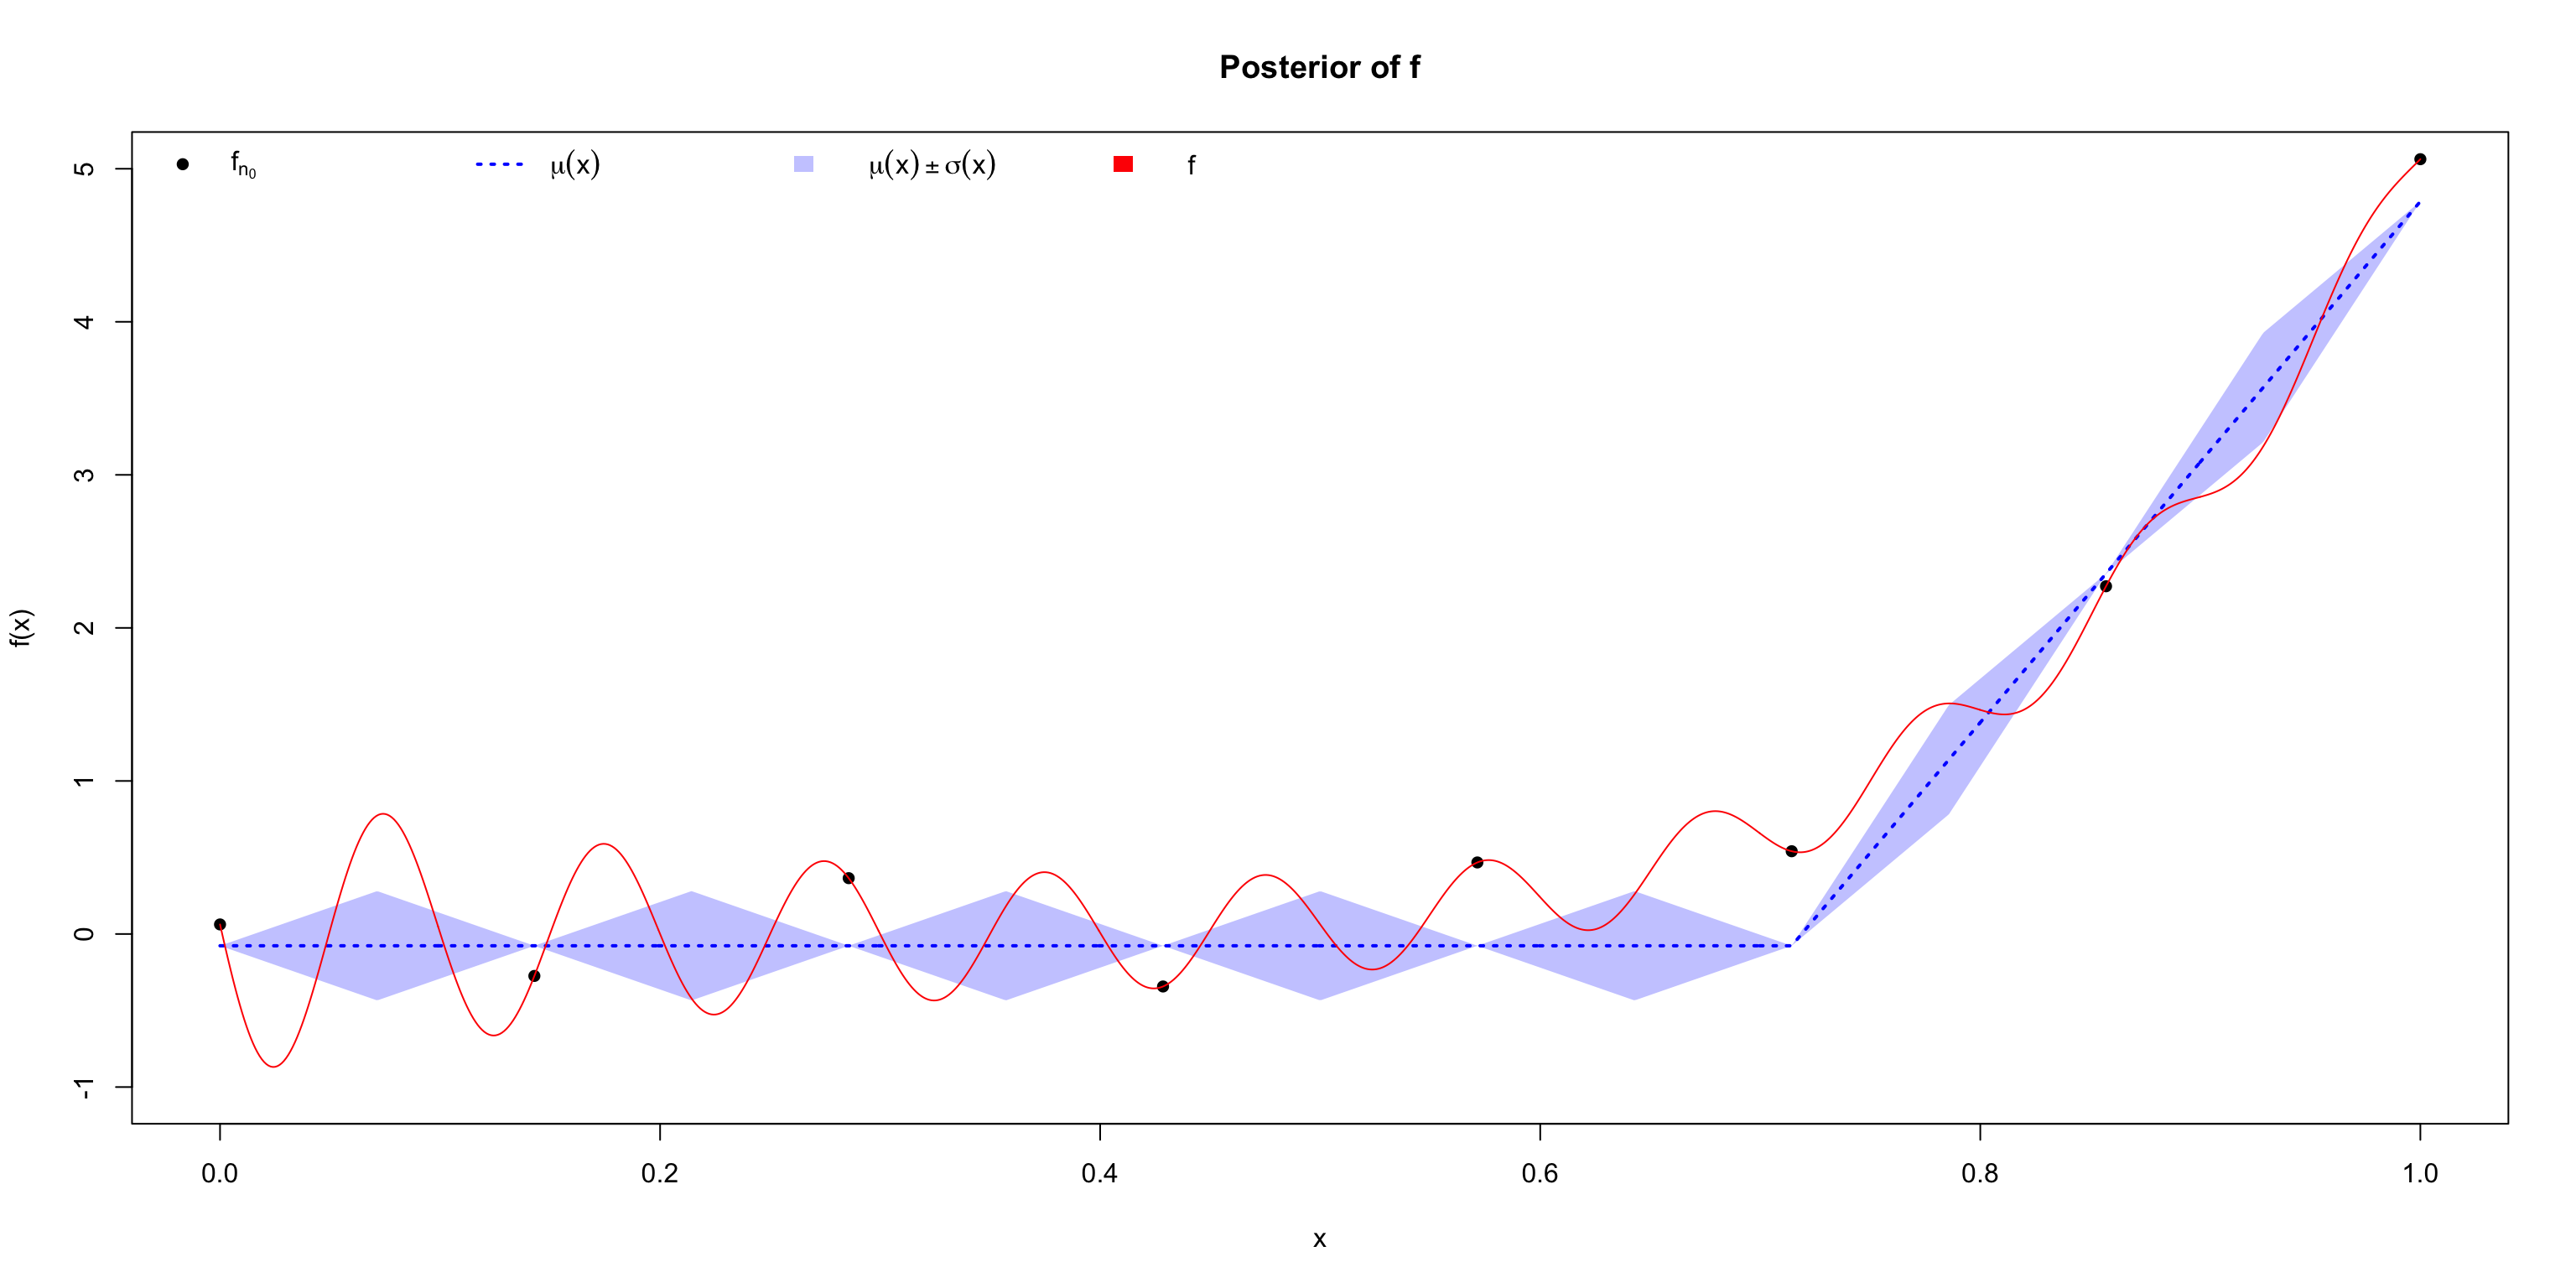
\includegraphics[width=8cm]{Figures/BASS8.png}
	\caption{A BASS posterior approximation of degree 1 to the Gramacy and Lee function \cite{gramacy2012cases} with 8 evaluations.}
	\label{gram8}
\end{figure}

\begin{figure}
	\centering
	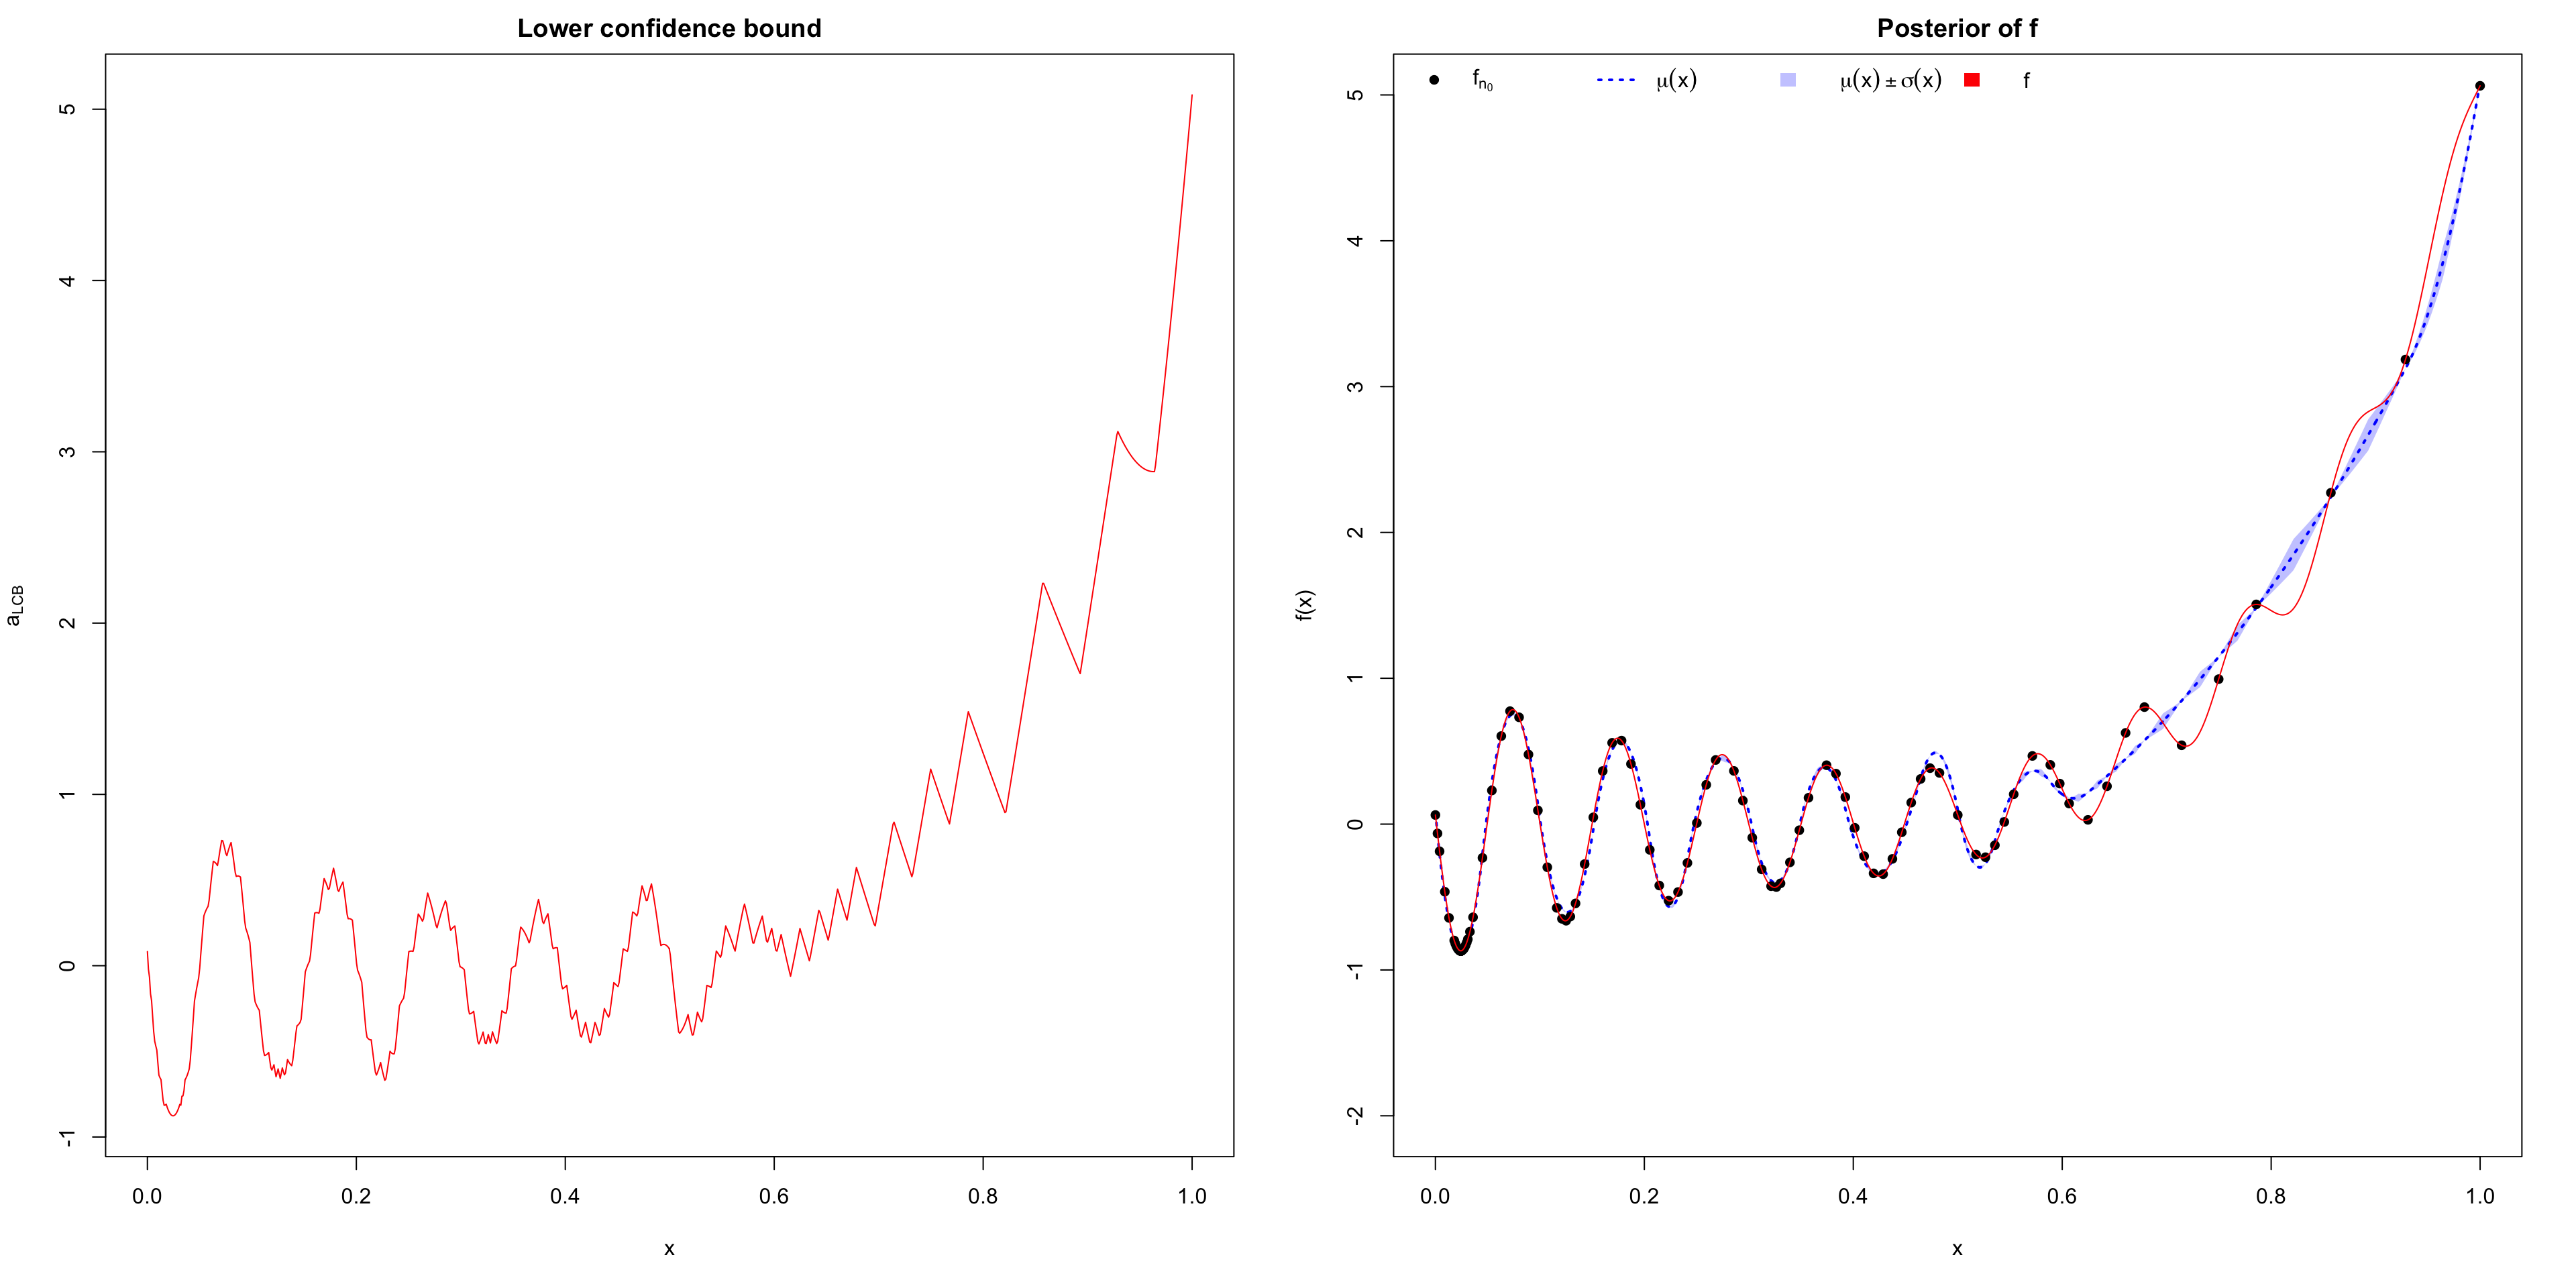
\includegraphics[width=8cm]{Figures/lowerbound.png}
	\caption{A BASS posterior approximation of degree 1 to the Gramacy and Lee function \cite{gramacy2012cases} with 115 total evaluations.}
	\label{gram115}
\end{figure}

While this initial plot does leave something to be desired, we notice that when we run BASS with 15 initial points and for 100 iterations for this same function, we get what is shown in Figure \ref{gram115}. We are using the lower confidence bound for the acquisition function in this case because it was relatively easy to evaluate.  



\section{Results for a One Dimensional Problem}

First, we note that we took the basis for this example from \onlinecite{boehmke2018uc} that can be loaded in R using the package \onlinecite{ameshouse}, AmesHousing. The dataset was originally published in \onlinecite{de2011ames}. For this dataset, we wish to predict the sale price of a house using an elastic net \cite{zou2005regularization} linear model, whose coefficients are calculated as 

\[ \hat \beta = \argmin_{\beta} ||y - \boldsymbol{X} \beta||^2 + \lambda \left( (1 - \alpha) ||\beta||_2^2 + \alpha||\beta||_1 \right), \]

where $\lambda$ is the penalty term, and $\alpha \in [0,1]$ specifies the mixture between the LASSO penalty and the Ridge penalty, where $\alpha = 0$ indicates a Ridge regression, and $\alpha = 1$ indicates a LASSO one. This type of problem lends itself extraordinarily well to finding optimal values for either $\lambda$, $\alpha$, or both. In this particular instance, we are training the regression model using the R package \textit{glmnet} \cite{glmnet}, and using the proposed method of Bayesian optimization with the BASS surrogate model to find the best value for $\alpha$, the mixture parameter in the model. 

While in the previous Figures we overlaid the real function over our estimation of the function and the specific points we had tested, we do not get that privilege in this case, as the function is costly to evaluate, and it would take several hours to have a good idea of the general function behaviour. Another interesting point is that while functions like the Gramacy and Lee function are smooth functions with little variance in their point evaluations when evaluating points that are close together, the functions we see in machine learning hyper-parameter tuning are much more volatile, so it is important to test the method on functions that truly represent what this method it is made to be used on. Another interesting difference is that while the regularized linear regression is trained on a portion of the data, we evaluate try and find the minimum sum of squared errors for a testing part of the dataset. 

\begin{figure}
	\centering
	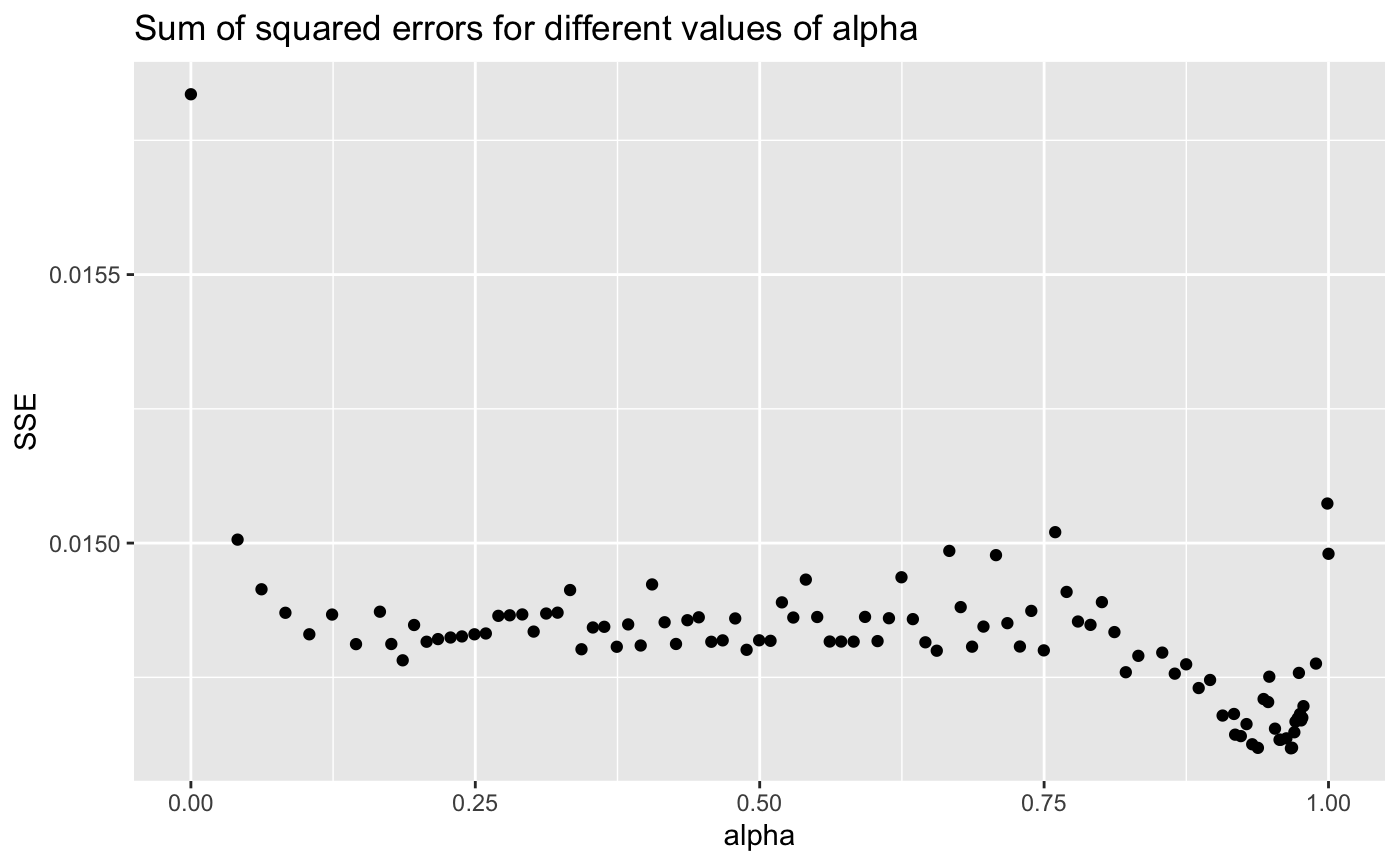
\includegraphics[width=8cm]{Figures/sse_alpha.png}
	\caption{Evaluations of the objective function for different values of $\alpha$.}
	\label{ssealpha}
\end{figure}

\begin{figure}
	\centering
	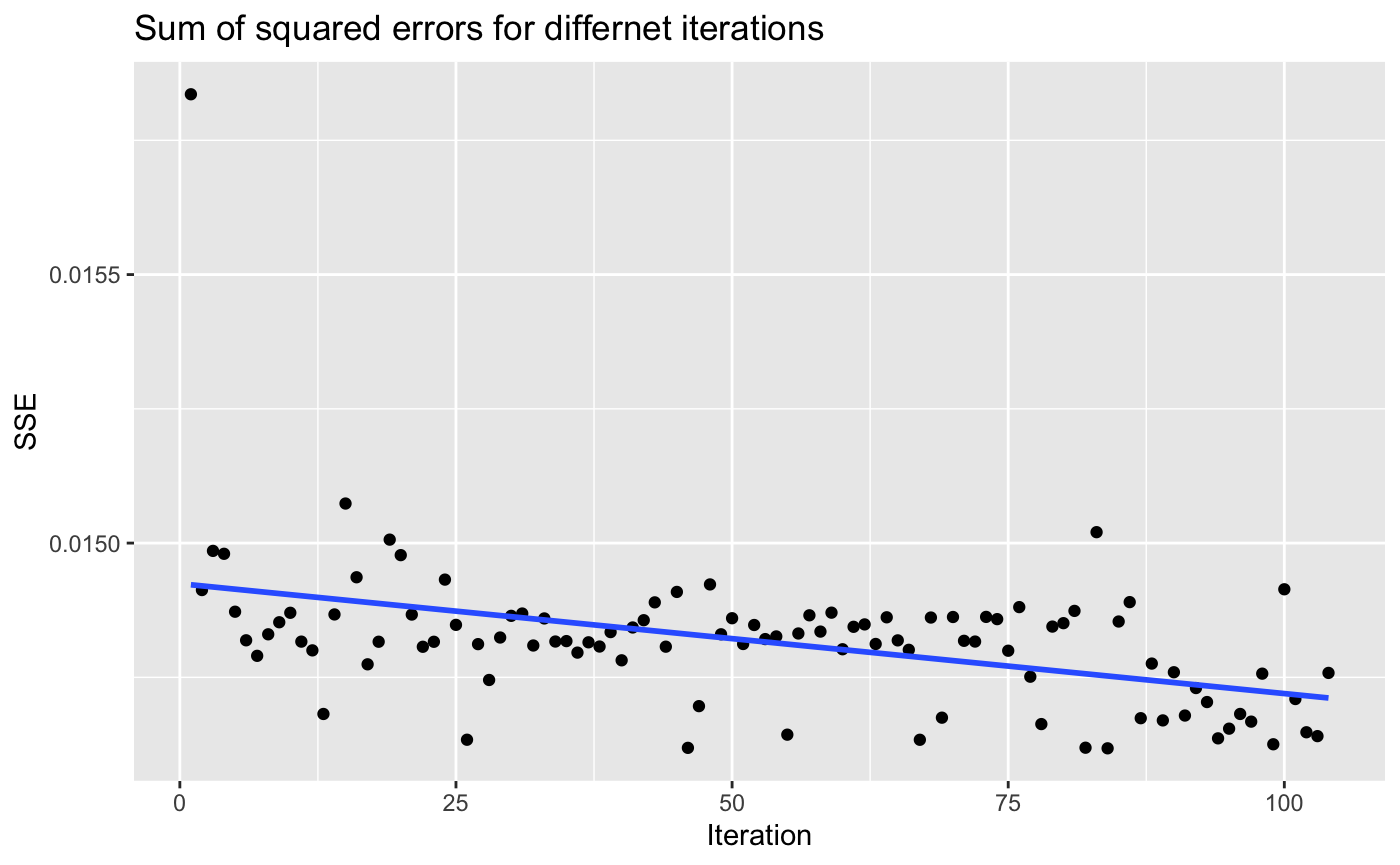
\includegraphics[width=8cm]{Figures/sse_iter.png}
	\caption{Evaluations of the objective function for different iterations of the algorithm.}
	\label{sseiter}
\end{figure}

In Figure \ref{ssealpha}, we can see the results of iterating through a Bayesian optimization algorithm with BASS as the surrogate model. Heuristically, we note that as we expected, we can see that the highest number of function evaluations are indeed being done in the area where the minimum found values have presented themselves, in this particular case, in the area approximately from $0.90$ to $0.98$.  In this case, we used a different acquisition, one based on the idea of probability of improvement \cite{snoek2012practical}. 

One interesting question that might be posed is if this is at all better than simply doing a grid search algorithm or randomly selecting points in the space. We present Figure \ref{sseiter}, where we can see that average the sum squared error goes down as the number of iterations goes up. That is to say, there is a relatively linear relationship in this case between the improvement we are seeing and the number of iterations that we let the algorithm run for. 

\section{Conclusions and further work}

This article is mostly just as a proof-of-work for what has been done up to now with regards to the BASS implementation as a surrogate model to turn into my Bayesian methods class (Hola, Alfredo!). There are some things missing to make this into a real paper, chief among them are: 
\begin{itemize}
	\item Formalizing a lot of the mathematical concepts in here and properly explaining a lot of the concepts and formulas that are mostly just glazed over.
	\item Implementing the case for categorical data, that is probably the biggest hole. 
	\item Research previous work and organize citations, with further mathematical rigidity, we need more citations. 
	\item Test out the Gaussian Process algorithm, and see the differences in convergence speed, and try out error estimation. 
\end{itemize}

The good news is that the heavy lifting in terms of programming is done. The various R programs that I use will be in the near future turned into functions for easier use, that is the next order of business. After that, implementing the categorical method in it's entirety, the one dimensional case I have but that is not super useful in practice, and then off to the races writing the article/thesis. 

\nocite{*}
\bibliography{aipsamp}% Produces the bibliography via BibTeX.

\end{document}
%
% ****** End of file aipsamp.tex ******